%
\chapter{Rekonstrukcija manevriranj plovila iz podatkov MEMS}
\label{Vaje:RekonsMems} % Always give a unique label

Na področju elektronike imamo vse več izjemno majhnih naprav, tako imenovanih \href{https://en.wikipedia.org/wiki/Microelectromechanical_systems}{\textit{MEMS}} naprav. V tej nalogi bodo imeli študentje opravka z MEMS napravo, ki bo vsebovala:
\begin{itemize}
	\item 3D magnetni kompas (Thin film magnetoresistive)
	\item 3D pospeškomer (MEMS solid state, capacitative readout)
	\item 3D žiroskop - "Rate of turn sensor - (rate gyroscope)" (MEMS solid state, monolithic, beam structure, capacitative readout)
	\item GPS (opcijsko)
\end{itemize}

\begin{figure}[!h]
	\centering 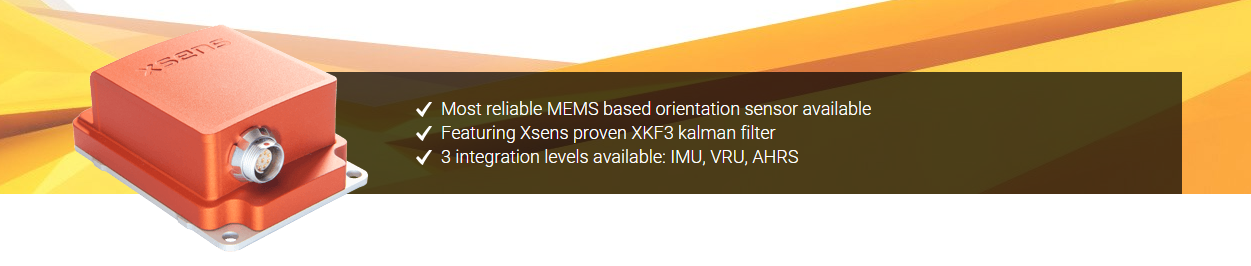
\includegraphics[width=12cm]{Vaje/ManevrZMems/figs/mems_photo.png}
	\caption{MEMS naprava proizvajalca \href{https://www.xsens.com}{Xens}.}
	\label{fig:v_mems_photo}
\end{figure}

S pomočjo te naprave bodo študentje dobili surove podatke o gibanju in jih grafično prikazali. S pomočjo grafov bodo ocenili in komentirali kaj se je med manevrom plovila dogajalo.

%Iz grafičnih prikazov rezultatov triosnih pospeškov, obračanj okoli osi in magnetnih gostot skpepajte kako se je plovilo gibalo! 

\section{Opis vaje}
\label{sec:v_mems_uvod}
Kot je bilo že napovedano bomo imeli opravka z elektronsko napravico, ki je sposobna več meritev hkrati. V škatlici, ki jo prikazana na sliki \ref{fig:v_mems_photo} imamo več senzorjev. Meritev se izvaja z različno frekvenco. Vse napravice so v danem trenutku v določenem statusu ali stanju. Znotraj naprave imamo poleg merilnih inštrumentov tudi tako imenovani "triger", ki sinhrono in ob točno določenem času pogleda na vse napravice in odčita podatke. Nato podatke primerno obdela in spravi skupaj v paketek. Nato paketek pošlje ven na izhod, na katerem imamo ponavadi priklopljen računalnik. Paketek je zapisan binarno z vnaprej določenim redom za posamezne bite.

\subsection{Opis naprave in priklop na računalnik}
Za napravo obstaja poseben kabel (glej sliko \ref{fig:v_mems_kit}), ki ga je potrebno ob priklopu na računalnik pravilno inštalirati. Če računalnik ob priklopu kabla ne razpozna kabla kot "Xens USB-serial converter" ~s pravilnim driverjem, je potrebno driver poiskati na spletu.

\begin{figure}[!h]
	\centering 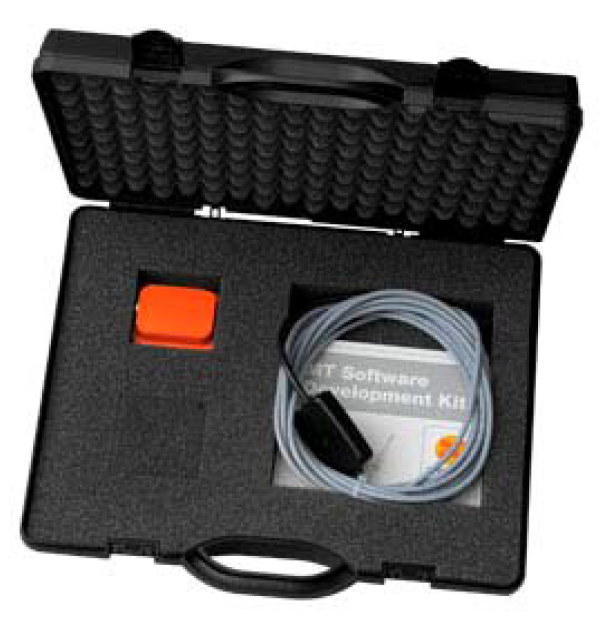
\includegraphics[width=12cm]{Vaje/ManevrZMems/figs/kit.png}
	\caption{MEMS naprava je v kovčku s kablom}
	\label{fig:v_mems_kit}
\end{figure}

Ko imate kabel sinhroniziran z računalnikom je potrebno inštalirati "Mt Manager". "MT Manager" je program s katerim zajemamo in prikazujemo podatke o napravi (glej sliko \ref{fig:v_mems_mt_gui} ) 

\begin{figure}[!h]
	\centering 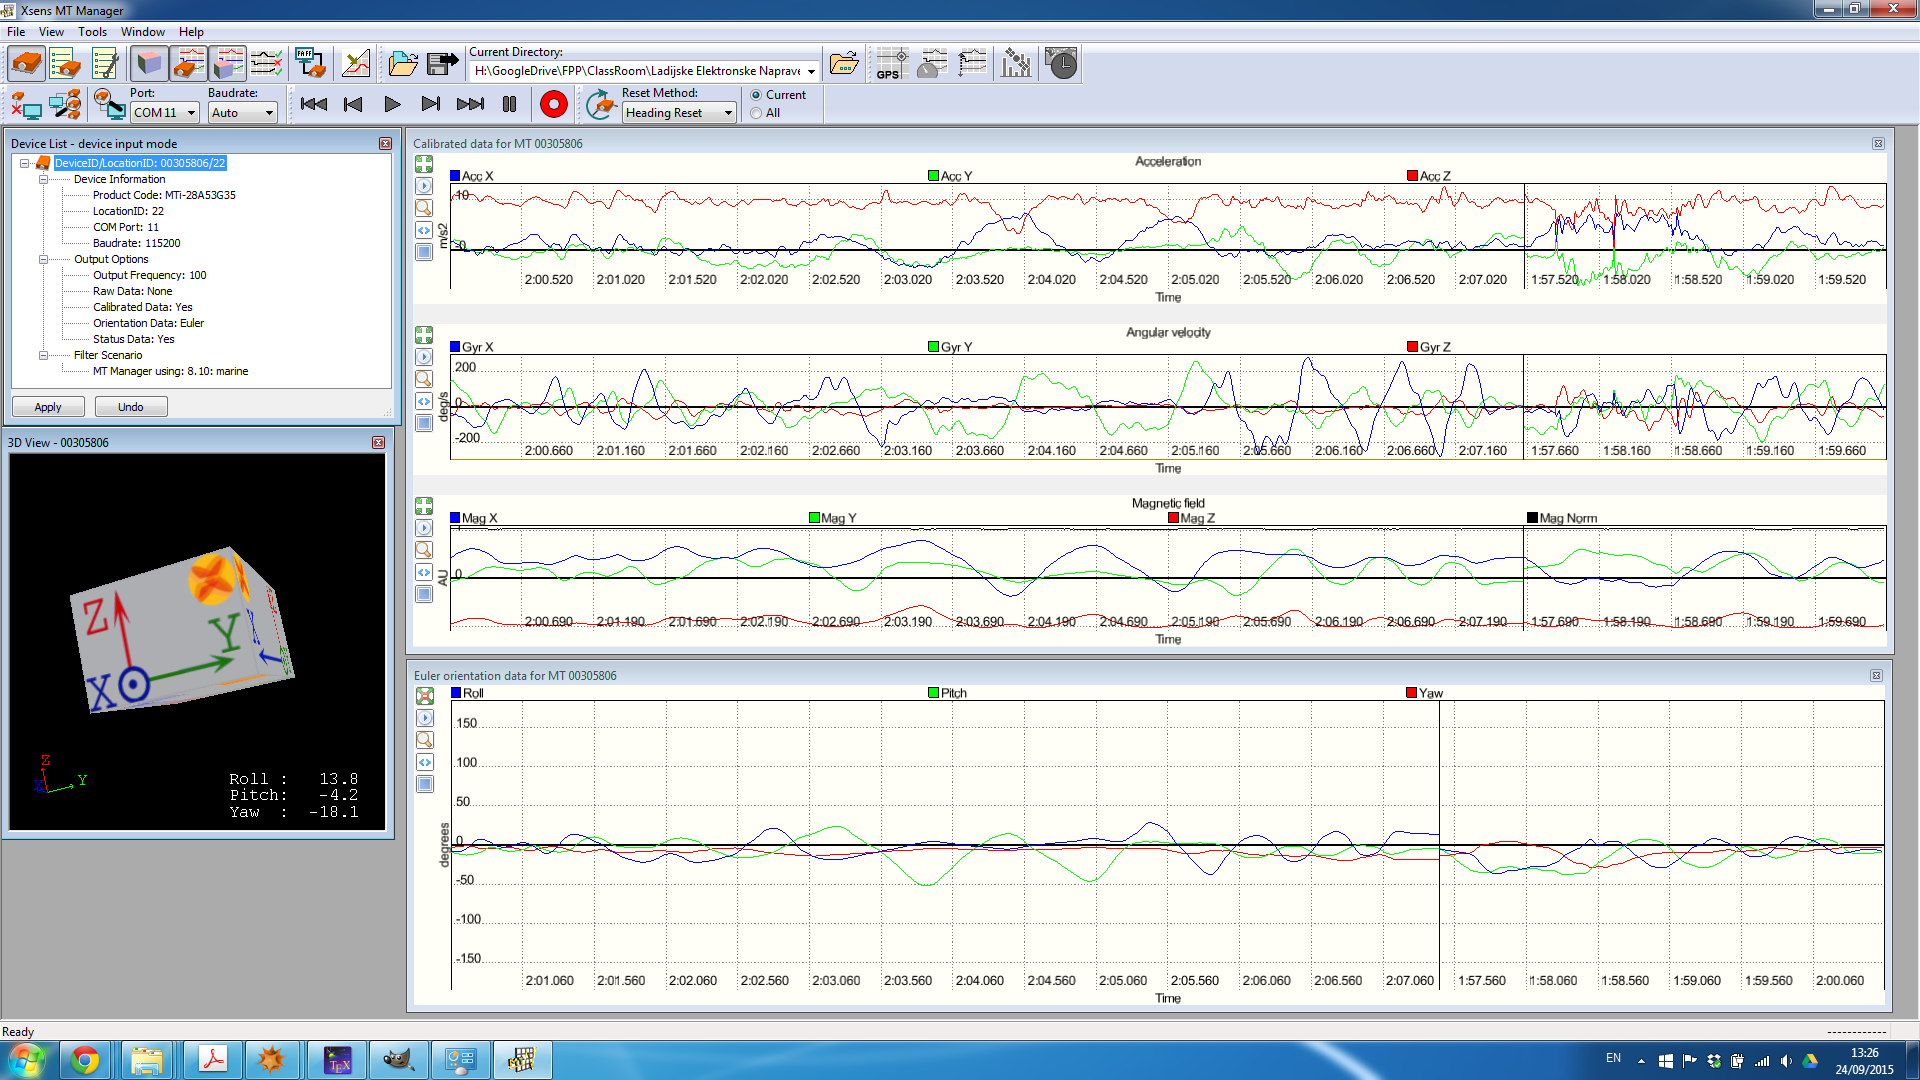
\includegraphics[width=12cm]{Vaje/ManevrZMems/figs/mt_manager_gui.png}
	\caption{MT Manager - GUI}
	\label{fig:v_mems_mt_gui}
\end{figure}

\noindent
Ena od vaših primarnih nalog bo spoznati program "MT Manager" in sicer:
\begin{itemize}
	\item znati nastaviti parametre za zajem podatkov,
	\item grafično pregledovati podatke,
	\item shranjevanje podatkov,
	\item izvoz podatkov za kasnejšo obdelavo.
\end{itemize}

\newpage
\subsection{Osnovne nastavitve "MT Manager-ja" - MTM}
Najprej napravo priklopite in zaženete MTM program. Ob zagonu bi moral napravo razpoznati in pričeti s konfiguracijo. Konfiguracija zajema tri korake, ki so prikazani na sliki \ref{fig:v_mems_mtm_cnfg}. Včasih se bo zgodilo, da MTM neha delovati. V tem primeru program izklopite in ponovno vklopite.

\begin{figure}[!htbp]
	\begin{minipage}{3.5cm}
		\centering 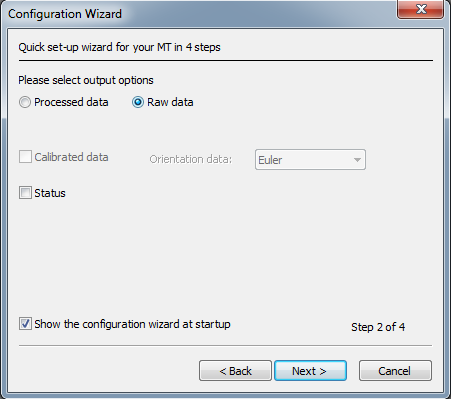
\includegraphics[width=4cm]{Vaje/ManevrZMems/figs/mtm_cnfg_01.png}
	\end{minipage}
	\hfill
	\begin{minipage}{3.5cm}
		\centering 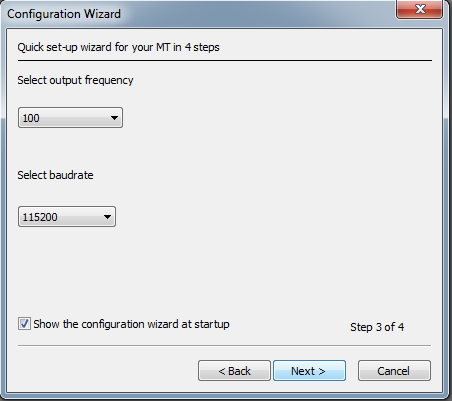
\includegraphics[width=4cm]{Vaje/ManevrZMems/figs/mtm_cnfg_02.png}
	\end{minipage}
	\hfill
	\begin{minipage}{3.5cm}
		\centering 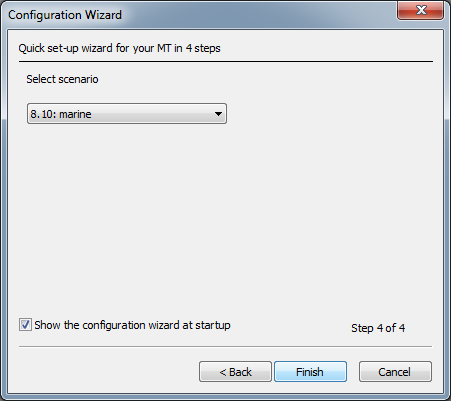
\includegraphics[width=4cm]{Vaje/ManevrZMems/figs/mtm_cnfg_03.png}
	\end{minipage}
	\caption{MT Manager - konfiguracija}
	\label{fig:v_mems_mtm_cnfg}
\end{figure}

Določene naloge bo potrebno naredi z dvema MEMS napravam hkrati. Nič težjega le obe napravi priklopite in zaženite MTM. Na sliki \ref{fig:v_mems_double} lahko vidite, kako izgleda spremljanje dveh naprav hkrati.

\begin{figure}[!h]
	\centering 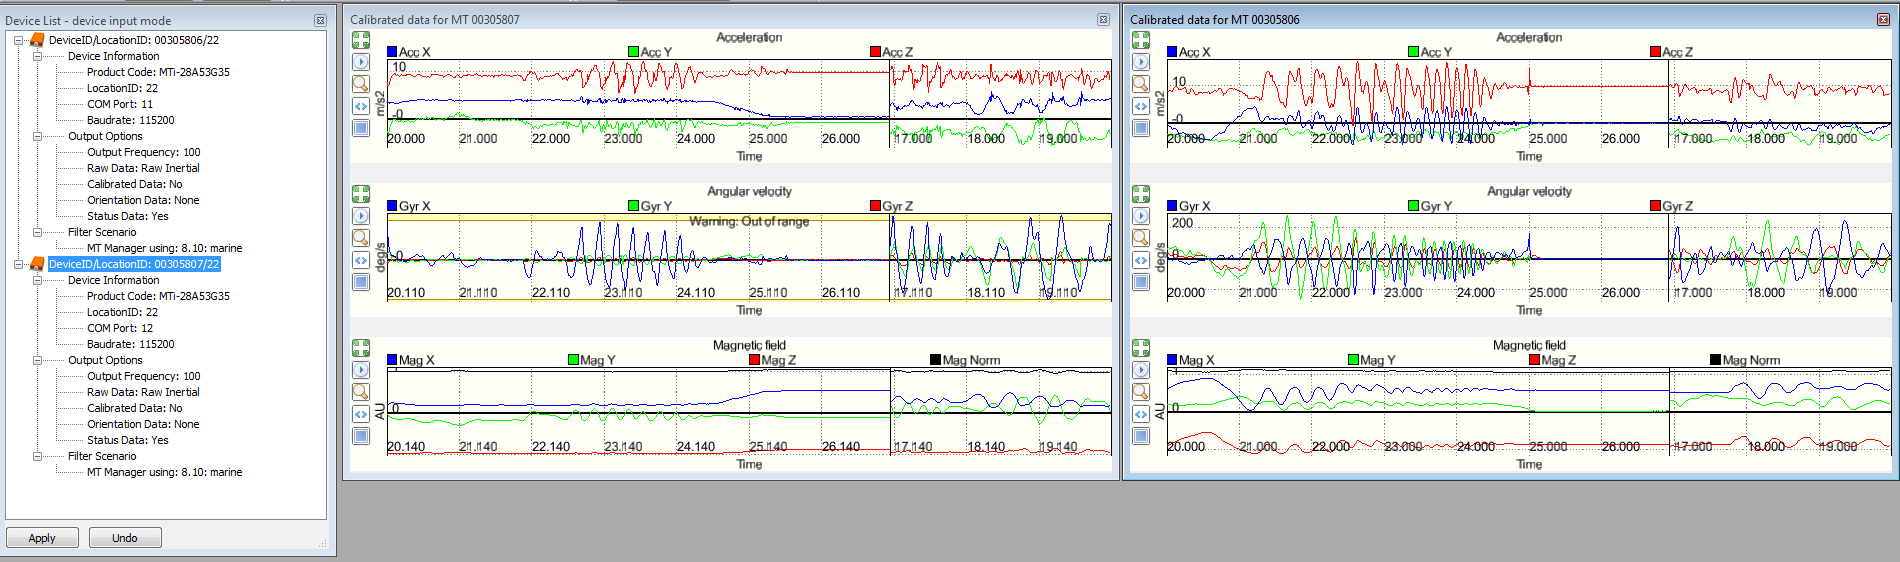
\includegraphics[width=12cm]{Vaje/ManevrZMems/figs/mtm_double.png}
	\caption{MTM z priključenima dvema napravama hkrati na PC.}
	\label{fig:v_mems_double}
\end{figure}

Naslednja faza je zajem podatkov. Podatke znotraj MTM programa zajamemo s pritiskom na tipko "Record" - to je rdeč disk z luknjo v "tool baru". Podatke bo shranjeval v datoteko z mtb končnico in so zapisani binarno. Za kasnejšo obdelavo podatke naložite v MTM (File$\to$Open) in jih izvozite (File$\to$Export) v ASCII format. Da bi imeli vse željene podatke morate nastaviti izvozni format (Tools$\to$Options) v obliki, ki jo kaže slika \ref{fig:v_mems_export}.

\begin{figure}[!h]
	\centering 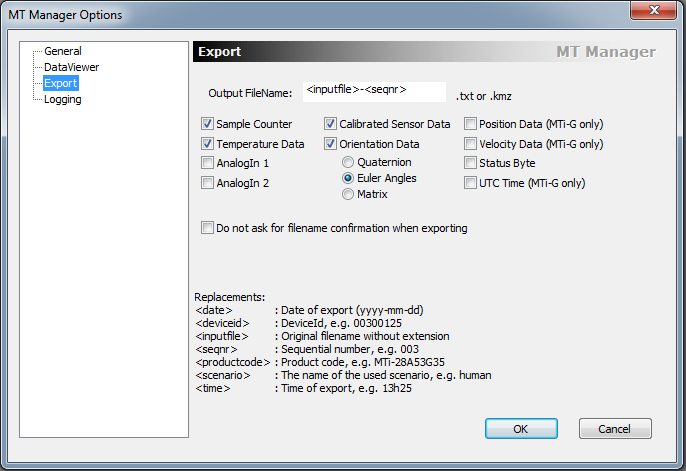
\includegraphics[width=6cm]{Vaje/ManevrZMems/figs/mtm_export.png}
	\caption{MTM nastavitev za izvoz podatkov.}
	\label{fig:v_mems_export}
\end{figure}

\newpage
Podatke boste dobili v datoteki s končnico txt, ki jo lahko uvozite v kateri koli program za obdelavo podatkov. Prvih nekaj vrstic izgleda takole:

\begin{figure}[!h]
	\centering 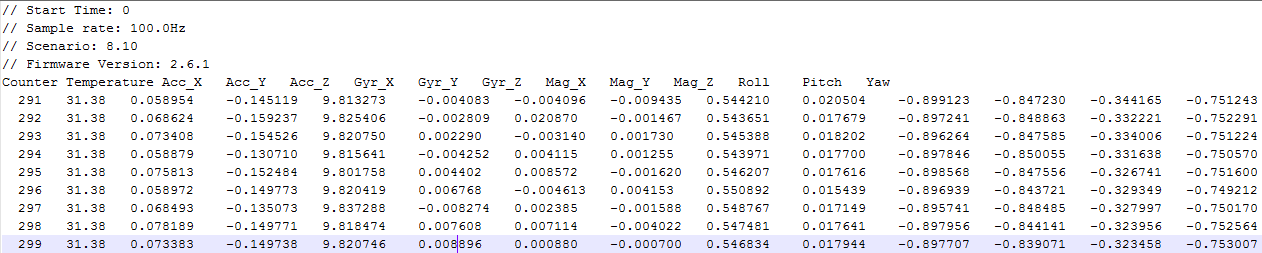
\includegraphics[width=12cm]{Vaje/ManevrZMems/figs/mtm_e_ascii.png}
	\caption{Izgled datoteke izvoza podatkov.}
	\label{fig:v_mems_e_ascii}
\end{figure}
\noindent
Ostale nastavitve MT Managerja si pa študentje razložijo sami s pomočjo literature, ki jo dobite pri mentorju.

\newpage
\section{Naloga}
Za vajo je potrebno izvesti več različnih manevrov recimo osmico, skok preko lastnega vala, ... Celoten manever je potebno shraniti v datoteko. Na kopnem je potrebno podatke izvoziti, obdelati in grafično prikazati. Kot primer si poglejmo grafe na sliki \ref{fig:v_mems_graf}. 

\begin{figure}[!htbp]
	\begin{minipage}{3.5cm}
		\centering 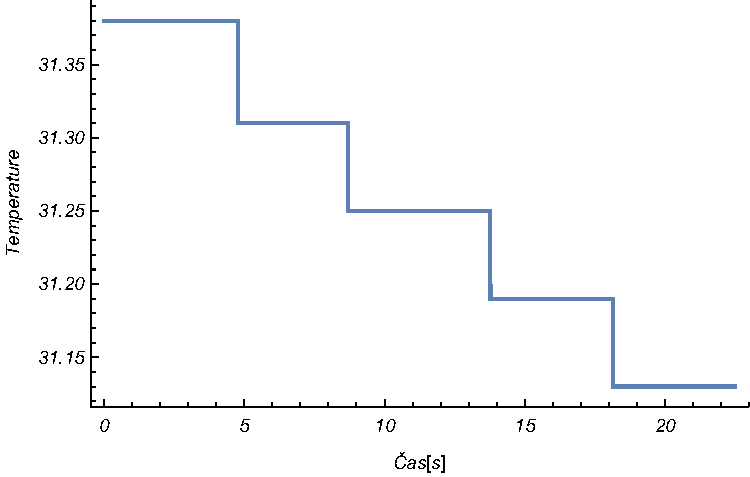
\includegraphics[width=4cm]{Vaje/ManevrZMems/figs/temp.pdf}
	\end{minipage}
	\hfill
	\begin{minipage}{3.5cm}
		\centering 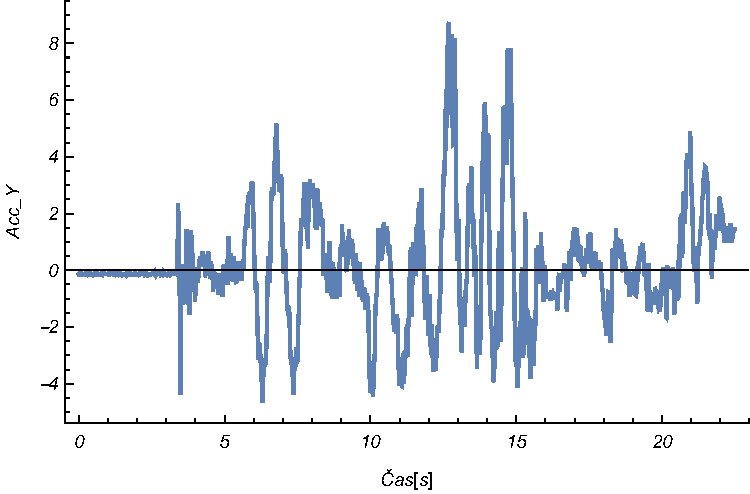
\includegraphics[width=4cm]{Vaje/ManevrZMems/figs/acc_y.pdf}
	\end{minipage}
	\hfill
	\begin{minipage}{3.5cm}
		\centering 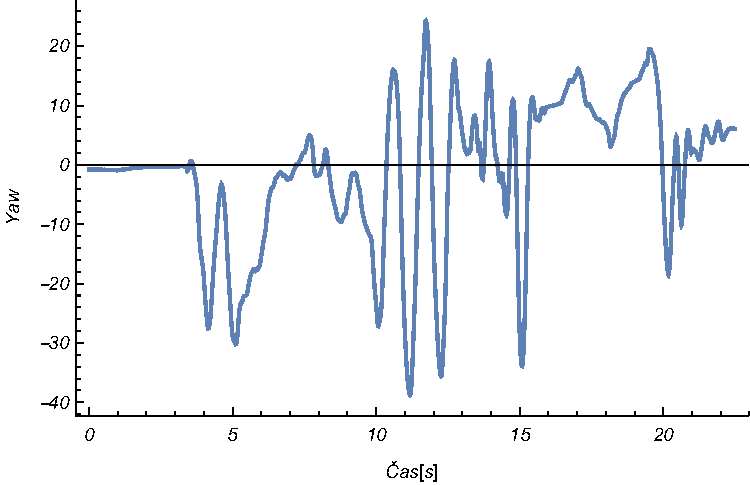
\includegraphics[width=4cm]{Vaje/ManevrZMems/figs/yaw.pdf}
	\end{minipage}
	\caption{Grafičen prikaz izvoznih podatkov temperature, pospeška v $y$ smeri in kota okoli $z$ osi - "Yaw".}
	\label{fig:v_mems_graf}
\end{figure}
